\documentclass[14pt]{beamer}
\usetheme{Antibes}
\definecolor{myOrange}{RGB}{238,97,53}
\setbeamercolor*{palette primary}{fg=myOrange}
\setbeamercolor*{palette secondary}{fg=myOrange,bg=white}
\setbeamercolor*{palette tertiary}{bg=myOrange,fg=white}
\setbeamercolor*{titlelike}{parent=palette primary}
\setbeamercolor*{itemize item}{fg=myOrange}
\setbeamercolor{block title example}{bg=myOrange} 
\setbeamercolor{section in toc}{fg=black}
\setbeamertemplate{sections/subsections in toc}[sections numbered]
\setbeamercolor{section number projected}{bg=myOrange,fg=yellow}
\setbeamertemplate{footline}[frame number]
\setbeamertemplate{frametitle}{
  \begin{centering}
  \insertframetitle
    \par
    \end{centering}
}
\setbeamertemplate{itemize item}{\textbullet}

\usepackage{tikz, tikz-qtree}
\usetikzlibrary{arrows, positioning}
\tikzset{node distance=0cm, auto}

\usepackage{amsmath}
\usepackage{ulem}
\usepackage{alltt}
\usepackage[english]{babel}
\usepackage{listings}
\usepackage{graphicx}
\definecolor{javared}{rgb}{0.6,0,0} % for strings
\definecolor{javagreen}{rgb}{0.25,0.5,0.35} % comments
\definecolor{javapurple}{rgb}{0.5,0,0.35} % keywords
\definecolor{javadocblue}{rgb}{0.25,0.35,0.75} % javadoc
\definecolor{javalinenumbers}{RGB}{79,80,81} % linenumbers
\definecolor{grey}{rgb}{0.95,0.95,0.95}
\lstset{language=Java,
basicstyle=\ttfamily \footnotesize,
keywordstyle=\color{myOrange}\textbf,
stringstyle=\color{javared},
commentstyle=\color{javagreen},
morecomment=[s][\color{javadocblue}]{/**}{*/},
numberstyle=\color{javalinenumbers}\tiny,
numbersep=10pt,
tabsize=4,
showspaces=false,
showstringspaces=false,
breaklines=true,
firstnumber=100,
backgroundcolor=\color{grey},
emph={
  val, var, def,
},
emphstyle=\color{myOrange}\bfseries,
morecomment=[s][\color{blue}]{@}{\ }
}

\definecolor{links}{HTML}{0000FF}
\hypersetup{colorlinks,linkcolor=,urlcolor=links}

\usepackage{hyperref}
\logo{
\includegraphics[width=1cm]{logo.png}}
\newcommand\B{\rule[-1.7ex]{0pt}{0pt}}
\def\colored#1{\textcolor{myOrange}{#1}}

\setcounter{tocdepth}{1}

\begin{document}
\title{Testing? Check It Out!}
\author{Arkady Galyash}
\institute{TosChart}
\date{\today}

\newcommand{\smaller}[1] {
  {\scriptsize {#1}}
}

% Здравствуйте, меня зовут Аркадий Галяш, я работаю в команде TosChart. 
% Сегодня я представляю вашему вниманию презентацию на тему "Java со ввкусом огурца", посвященную проблемам и преимуществам использования инструментария BDD в реальных проектах
% Вопросы можно задавать как походу доклада, так и в конце.
\frame{\titlepage}

\frame%
{\frametitle{Agenda}
  \tableofcontents[1]
}

\section{How regular JUnit test looks like (in time)?}
\subsection{Intro}
\frame{\frametitle{Intro}
  \begin{itemize}
    \item John Doe The Programmer
    \item Java developer @ Moon Ms
    \item Since 2000
    \item Binary search algorithm
  \end{itemize}
}

\subsection{June 2000}
\frame{\frametitle{June 2000}
  \begin{center}
    
\includegraphics[width=0.4\textwidth]{2000.png} \\
    Just graduated, "tests are for chicken"
  \end{center}
}

\subsection{May 2001}
\frame{\frametitle{May 2001}
  \begin{center}
    
\includegraphics[width=0.4\textwidth]{2001.png} \\
    JUnit discovered
  \end{center}
}

\subsection{July 2006}
\frame{\frametitle{July 2006}
  \begin{center}
    
\includegraphics[width=0.4\textwidth]{2006.png} \\
    User tries to search non-existant element
  \end{center}
}

\subsection{December 2007}
\frame{\frametitle{December 2007}
  \begin{center}
    
\includegraphics[width=0.4\textwidth]{2007.png} \\
    User tries to search in array with duplicates
  \end{center}
}

\subsection{October 2009}
\frame{\frametitle{October 2009}
  \begin{center}
    
\includegraphics[width=0.4\textwidth]{2009.png} \\
    Integer overflow
  \end{center}
}

\subsection{Summary}
\begin{frame}[t]
  \frametitle{Long way}
  \begin{center}
    \begin{tikzpicture}
      \node[inner sep=0pt] at (0,4.25)
        {
\includegraphics[width=2cm]{2000.png}};
      \node[inner sep=0pt] at (2,4.25)
        {
\includegraphics[width=2cm]{2001.png}};
      \node[inner sep=0pt] at (4,4.25)
        {
\includegraphics[width=2cm]{2006.png}};
      \node[inner sep=0pt] at (6,4.25)
        {
\includegraphics[width=2cm]{2007.png}};
      \node[inner sep=0pt] at (8,4.25)
        {
\includegraphics[width=2cm]{2009.png}};
      \node (s1) at (8, 0) {};
      \node (s2) at (6, 0.5) {};
      \node (s3) at (4, 1) {};
      \node (s4) at (2, 1.5) {};
      \node[draw=none] at (0,2.5) {2000};
      \node[draw=none] at (2,2.5) {2001};
      \node[draw=none] at (4,2.5) {2006};
      \node[draw=none] at (6,2.5) {2007};
      \node[draw=none] at (8,2.5) {2009};
      \draw[thick,->] (s1) -- (9,0); 
      \draw[thick,->] (s2) -- (9,0.5);
      \draw[thick,->] (s3) -- (9,1);
      \draw[thick,->] (s4) -- (9,1.5);
      \node[left=0.1cm of s1] {\footnotesize hugeArrayTest};
      \node[left=0.1cm of s2] {\footnotesize sameTest};
      \node[left=0.1cm of s3] {\footnotesize missingTest};
      \node[left=0.1cm of s4] {\footnotesize simpleTest};
      \fill(2,1.5) circle (2pt);
      \draw (4,1.5cm+2pt) -- (4,1.5cm-2pt);
      \draw (6,1.5cm+2pt) -- (6,1.5cm-2pt);
      \draw (8,1.5cm+2pt) -- (8,1.5cm-2pt);
      \fill(4,1) circle (2pt);
      \draw (6,1cm+2pt) -- (6,1cm-2pt);
      \draw (8,1cm+2pt) -- (8,1cm-2pt);
      \fill(6,0.5) circle (2pt);
      \draw (8,0.5cm+2pt) -- (8,0.5cm-2pt);
      \fill(8, 0) circle (2pt);
    \end{tikzpicture}
  \end{center}
\end{frame}

\frame{\frametitle{xUnit}
  \begin{itemize}
    \item Design tests example by example
    \item Test suites give us confidence that code works for the examples we thought of
    \item If we discover a test case, this test is useless right now, it may be useful only in future
    \item "Don't ask, don't tell"
  \end{itemize}
}

\section{Property based testing}
\frame{\frametitle{Property based testing}
  \begin{itemize}
    \item Another approach
    \item You specify actions and post-conditions 
    \item Let computer generate input data \\ (it will not forget about corner cases)
  \end{itemize}
}

\subsection{QuickCheck}
\frame{\frametitle{QuickCheck History}
  \begin{itemize}
    \item Initially written for Haskell in 1999
    \item By Koen Claessen and John Hughes
    \item BSD-style License
  \end{itemize}
}

\frame{\frametitle{QuickCheck implementations}
  \begin{center}
    
\includegraphics[width=0.9\textwidth]{all_checks.png}
  \end{center}
}

\section{Java Quickchecks}
\frame{\frametitle{QuickCheck implementations}
  \begin{center}
    
\includegraphics[width=0.9\textwidth]{jvm_checks.png}
  \end{center}
}


\frame{\frametitle{Scala? Clojure?}
  \begin{center}
    
\includegraphics[width=0.8\textwidth]{no_thanks.jpeg}
  \end{center}
}

\frame{\frametitle{Implementations criteria}
  \begin{itemize}
    \item Generators of custom types
    \item Generators with restrictions
    \item Search-space customization
  \end{itemize}
}

\frame{\frametitle{Trie}
  \begin{center}
  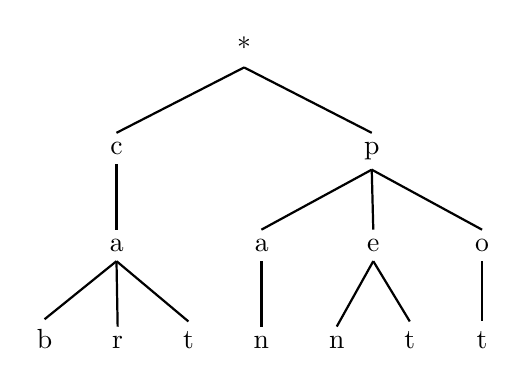
\begin{tikzpicture}
    \tikzset{level distance=3.5em, sibling distance=1.5em, edge from parent/.append style={thick} }
    \Tree [.* [.c [.a b r t ] ] [.p [.a n ] [.e n t ] [.o t ] ] ]
  \end{tikzpicture}
  \end{center}
}

\subsection{junit-quickcheck}
\frame{\frametitle{junit-quickcheck}
  \begin{itemize}
    \item Based on \texttt{org.junit.experimental.theories.*}
    \item Annotation-based
    \item On \href{https://github.com/pholser/junit-quickcheck}{github.com} by @pholser
    \item 0.3 version in maven repository
    \item Found \href{https://github.com/pholser/junit-quickcheck/issues/35}{bug with generics} during making presentation
  \end{itemize}
}

\frame{\frametitle{Demo}
  \begin{center}
    
\includegraphics[height=0.8\textheight]{not_ready.jpg}
  \end{center}
}

\subsection{JCheck}
\frame{\frametitle{JCheck}
  \begin{itemize}
    \item Has its own JUnit Runner
    \item Annotation-based
    \item On \href{http://sourceforge.net/projects/jcheck/}{sf.net} by @hampusr
    \item 0.1 version jar from 2008
  \end{itemize}
}

\frame{\frametitle{Demo}
  \begin{center}
    
\includegraphics[height=0.8\textheight]{show_code.jpg}
  \end{center}
}

\subsection{quickcheck}
\frame{\frametitle{quickcheck}
  \begin{itemize}
    \item Do not have Runner at all
    \item Handle only data generation
    \item On \href{https://bitbucket.org/blob79/quickcheck}{bitbucket.org} by @blob79
    \item 0.6 version in maven repository
  \end{itemize}
}

\frame{\frametitle{Demo}
  \begin{center}
    
\includegraphics[height=0.8\textheight]{finally.jpeg} 
  \end{center}
}

\section{Where can we use it?}
\frame{\frametitle{ThinkScript}
  \begin{itemize}
    \item Programming language for traders
    \item Technical analisys
    \item Has a lot of built-in functions (SMA, EMA, WMA, ...)
  \end{itemize}
}

\frame{\frametitle{Standard deviation}
  \begin{center}
    \Large{$\sigma = \sqrt{\frac{1}{N} \sum_{i=1}^N (x_i - \mu)^2}$, \\
    $\mu = \frac{1}{N} \sum_{i=1}^N x_i$}
  \end{center}
}

\frame{\frametitle{Demo}
  \begin{center}
    
\includegraphics[height=0.8\textheight]{we_can.png} 
  \end{center}
}

\frame{\frametitle{Donald Knuth is shocked by stdev}
  \begin{center}
    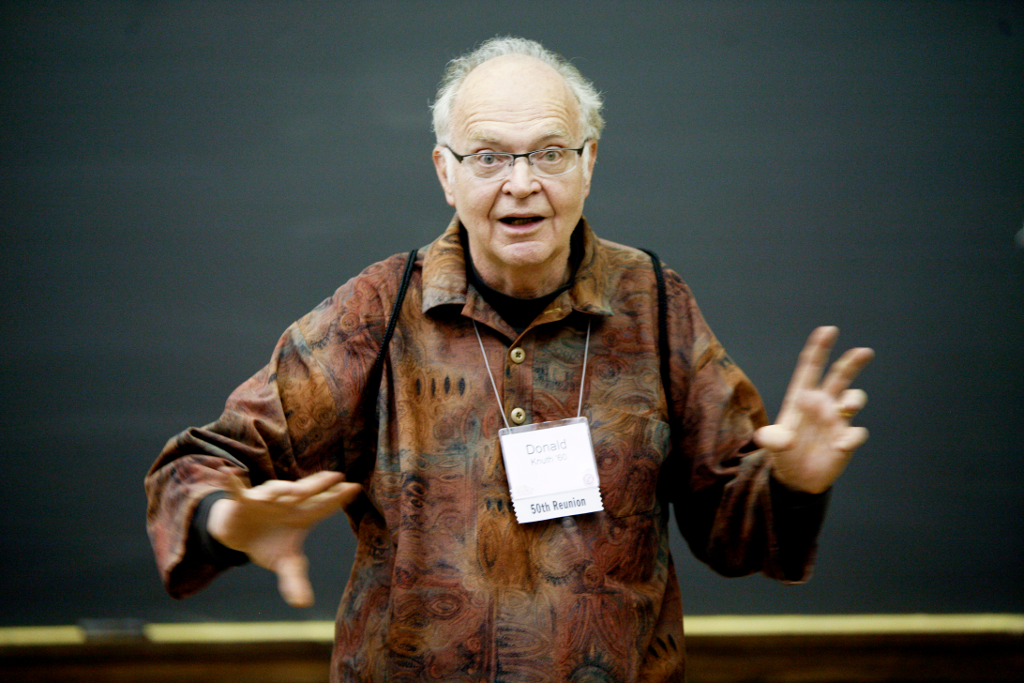
\includegraphics[width=0.8\textwidth]{knuth.jpg} 
  \end{center}
}
% Ссылки 
\section{Links}
\frame{\frametitle{Links}
  \begin{itemize}
    \item \href{https://github.com/gark87/job-misc/tree/master/presentations/check_it_out/JohnDoeProject}{JohnDoeProject with examples} $\vcenter{\hbox{
\includegraphics[width=2.5em]{github.png}}}$
    \item \href{http://www.haskell.org/haskellwiki/Introduction_to_QuickCheck2}{Introduction to QuickCheck2}
    \item \href{http://theyougen.blogspot.ru/search/label/quickcheck}{Blog dedicated to Java Quickcheck}
    \item \href{http://thinkrelevance.com/blog/2013/11/26/better-than-unit-tests}{Better Than Unit Tests}
  \end{itemize}
}
\frame{\frametitle{Thank you!}
  \begin{center}
    
\includegraphics[height=0.8\textheight]{last.jpg}
  \end{center}
}

\end{document}
